\section{Audio Transmission Measurement}
This second major category of VNA measurements consists of generating a sine wave and applying this to some form of network.
 The network must have at least two sets of connections that act as the input and output.
The transmission measurement measures the input and output voltages and finds the ratio of the voltage magnitudes along with the difference in phase.
%
\subsection{Description}
\textbf{Complex Transmission - }The concept of voltage gain  is common.
This is directly applied here when we take the ratio of the magnitude of the outpurt voltage to that of the input voltage.
That measure does not involve the phase of the signals and is the same as applying a portable DVM to the terminals and dividing the result with a calculator.
The "complex" or "vector" part comes in with phase measurement.
Wth our VNA, we determine how much phase difference there is with the input and output sine waves.
This can be important for equipment such as  filters, control systems or communications networks.
It also is part of allowings a complete mathematical model of linear circuits to be constructed .  This can be a valuable tool for design of circuits.

It is worth noting that some of the concepts such as scattering parameters and reflection coefficients are applicable at low frequencies though they may be mainly thought of as RF descriptors.  Complex transmission (and impedance) measurements support these descriptors.  We won't attempt to cover all the possibilities here, but it would be an interesting topic for someone to explore.

%\textbf{Measurement Transmission - }

\subsection{Instructions}
\textbf{Getting Started - }This procedure parallels the impedance measurements of the previos section.  We will cover the essence of a transmission measurement using the touch screen.
Everything covered here, and more, can be done via the USB-Serial link, as is described in the "AVNA Serial Control" section.

When the AVNA is powered up you have a choice of four Audio Test Instruments along with Service and Calibration functions as was shown before in Figure \ref{AVNA_000-label}.

\begin{figure}[H]
\begin{center}
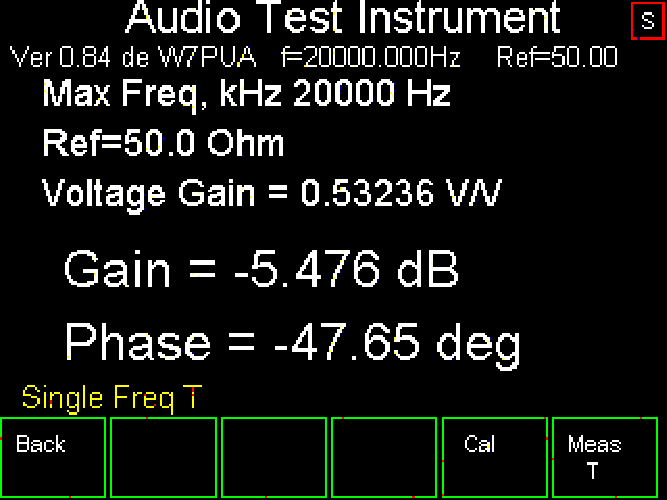
\includegraphics[scale=0.75]{./images/AVNA_029.pdf}
\caption{AVNA Transmission measurement for a single frequency.}
\label{AVNA_029-label}
\end{center}
\end{figure}
%
Referring to Figure \ref{AVNA_000-label}, we are now at the main Audio Test Instrument home screen.
We used to call this just, "the AVNA," but now we have added the other instruments like the Spectrum Analyzer, so this needs more descriptors.
For our impedance measurements, we will select the menu item, "AVNA" by touching that box at the bottom of the screen.
That  covers everything for the current discussion, leading to the AVNA main screen.

\begin{figure}[H]
\begin{center}
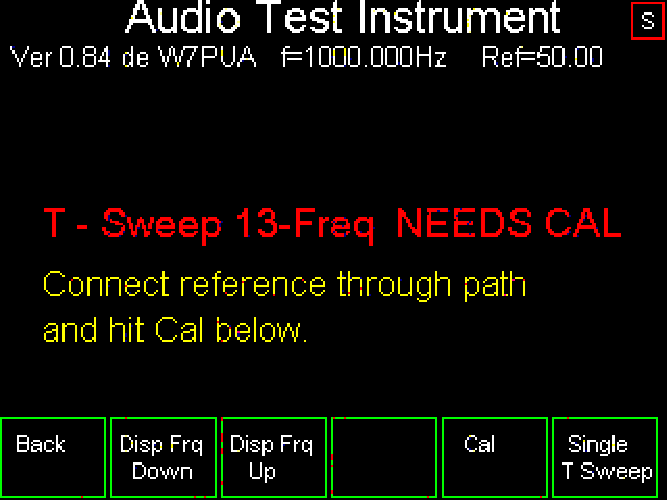
\includegraphics[scale=0.75]{./images/AVNA_031.pdf}
\caption{AVNA Transmission showing need for calibration.}
\label{AVNA_031-label}
\end{center}
\end{figure}
%

\begin{figure}[H]
\begin{center}
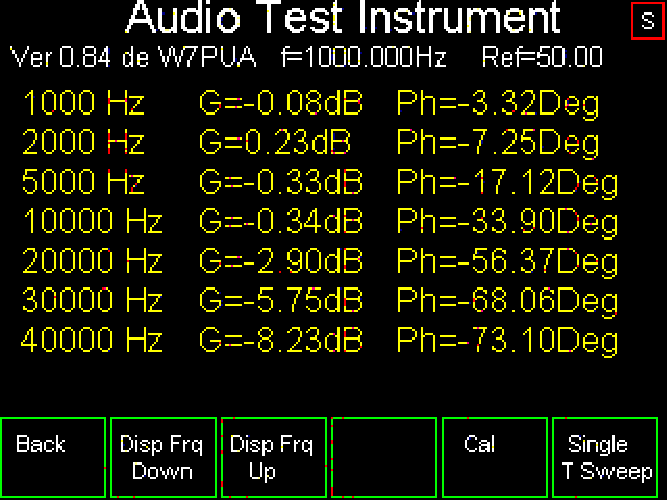
\includegraphics[scale=0.75]{./images/AVNA_032.pdf}
\caption{AVNA Swept Transmission measurement screen.}
\label{AVNA_032-label}
\end{center}
\end{figure}
%
\subsection{Discussion}
xxx
